\chapter{Méthodes de classification des données}\label{classif}
    Ce chapitre a pour but la sélection d'une ou plusieurs techniques de classification visant à
    attribuer la valeur 0 ou 1 à une classe que l'on créera et ajoutera aux ensembles
    $\mathbb S_{etr}$.

    Pour confirmer les propos tenus ici, l'équipe se base principalement sur les pages Wikipedia
    des modèles concernés~\textit{(\cite{wikiRL, wikiBN, wikiKNN, wikiTrainingValidationTest})} et sur la littérature
    d'introduction au Machine Learning~\textit{(\cite{introML, MLFondamentaux})}.

    L'article expliquant le fonctionnement et l'intérêt du modèle DoppelGanger~\textit{(
    \cite{doppelGANger})} est un autre guide pour la réflexion. On peut en effet en extraire
    cette figure :

    \begin{figure}[H]
        \centering
        {\fbox{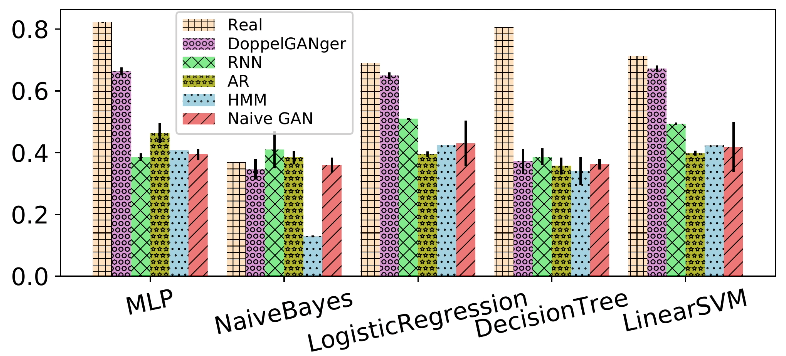
\includegraphics[width = 0.8\textwidth]{figures/Resultats/ChapitreDopelGanger/dopelClassifiyingSets}}}
        \caption{Taux de succès de différents modèles de classification, comparaison entre le DoppelGanger et d'autres générateurs}\label{fig:ganclassifs}

    \begin{tcolorbox}[colback=linkborder_Color!5!white,colframe=linkborder_Color!75!black]
        Une détermination rigoureuse d'un modèle de classification voudrait que l'on étudie
        également le meilleur ratio de membres et de non-membres.
        \textit{(autrement dit de lignes labellées "0" et "1")}. On fait cependant l'hypothèse
        que les tâches $\mathbb C_{T_i}$ comportent autant de membres que de non-membres.

        Ainsi, on définit :
        \begin{equation}
            \mathbb{S}_{etr} = \mathbb{S}'_{pub} + \mathbb{S}'_{priv} \, \Bigm \lvert \, l
            \left( \mathbb{S}'_{pub} \right) = l\left( \mathbb{S}'_{priv} \right)
        \end{equation}
        Avec $\mathbb{S}'_{pub}$ composé de lignes choisies aléatoirement dans $\mathbb{S}_{pub}$ mais n'appartenant pas à $\mathbb{S}'_{priv}$.
    \end{tcolorbox}

    \end{figure}
    \newpage\section{Choix de l'algorithme}

        Le meilleur modèle à utiliser pour classifier $\mathbb C_{T_i}$ dépend de nombreux
        paramètres. Une longue partie du projet a été consacrée à la détermination de ce modèle
        en amont de son application à la compétition.
        Le retour d'expérience montre qu'il est en réalité préférable d'utiliser de nombreux modèles
        et de comparer leurs performances sur des cas concrets. En effet, les classifieurs
        proposés par \texttt{scikit-learn} sont conçus pour être utilisés en série,
        indépendamment de leur fonctionnement interne, et leur temps de calcul est raisonnable.

        Les modèles retenus sont ceux présentés dans les tableaux \ref{tab3:}, \ref{tab2:} et \ref{tab:}\footnote{Un classifieur dit "empileur" prend les prédictions produites par d'autres modèles pour faire sa propre prédiction d'une cible ou d'un label.\textit{(\cite{MLFondamentaux}, Chapitre 3)}}.


        \begin{tcolorbox}[colback=linkborder_Color!5!white,colframe=linkborder_Color!75!black]
            Pour des raisons de simplicité, l'équipe n'a pas utilisé de réseaux de neurones pour
            la classification des données. Toutefois, on peut également justifier ce choix en
            considérant que pour un problème de classification binaire de séries temporelles,
            les algorithmes traditionnels de Machine Learning sont \textit{a priori} efficaces.
        \end{tcolorbox}
    \section{Évaluation des classifieurs}

        \subsection{Choix des métriques}

            Il est important de choisir plusieurs paramètres pour apprécier finement le
            comportement des classifieurs. Le premier utilisé par l'équipe est la matrice de
            confusion, que l'on normalise vis-à-vis de la taille du dataset de test. La matrice
            de confusion idéale est donc :

            \begin{equation}
                M_c = \begin{pmatrix}
                    0,5 && 0\\
                    0 && 0,5
                \end{pmatrix}
            \end{equation}
            \myequations{Matrice de confusion idéale après normalisation des proportions sous l'hypothèse d'équilibre des classes}

            On calcule également les score de précision et de rappel pour tenir compte de
            l'influence de faux positifs et de faux négatifs respectivement :

            \begin{equation}
                \mathrm{precision}=\frac{1}{1+\displaystyle{\frac{\tau_{fp}}{\tau_{tp}}}}
            \end{equation}
            \myequations{Score de précision d'une classification}

            \begin{equation}
                \mathrm{rappel}=\frac{1}{1+\displaystyle{\frac{\tau_{fn}}{\tau_{tp}}}}
            \end{equation}
            \myequations{Score de rappel d'une classification}

            On calcule de plus le score $f_1$, moyenne harmonique de la précision et du rappel.

            \begin{equation}
                f_1=\frac{2\times \tau_{tp}}{2\times \tau_{tp} + \tau_{fp} + \tau_{fn}}
            \end{equation}
            \myequations{Score $f_1$ d'une classification}

            Enfin, on calcule l'aire sous la courbe ROC de la classification.

            \begin{figure}[H]
                \centering
                \fbox{
                    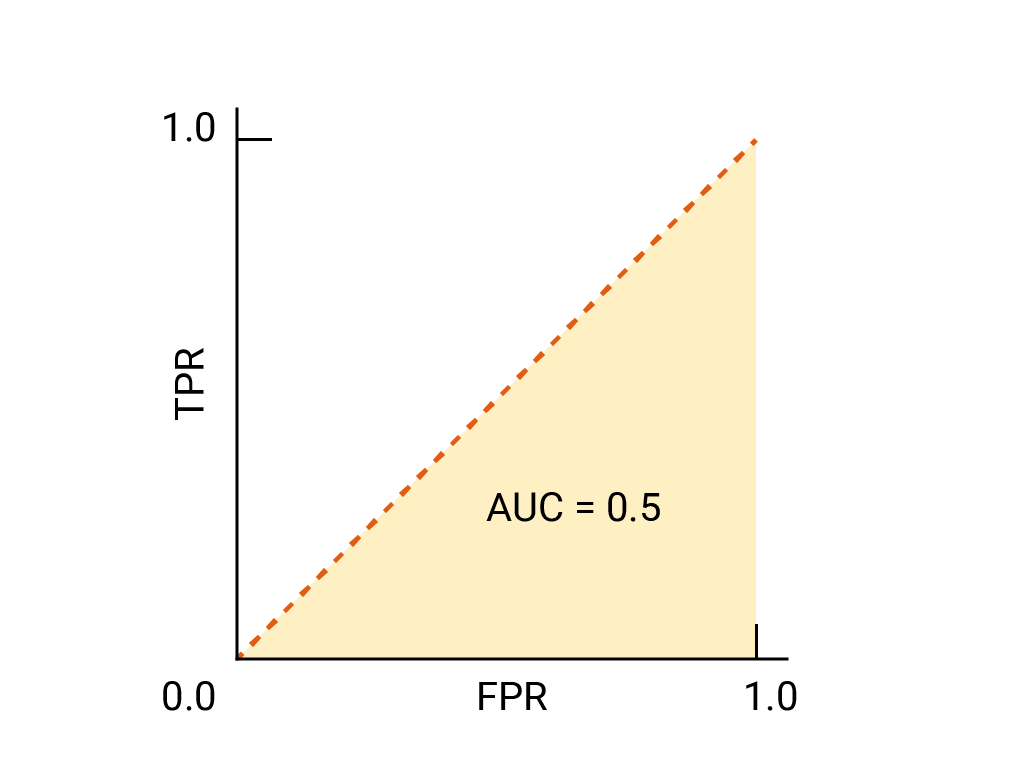
\includegraphics[width = 0.25\textwidth]{figures/schemas/auc_0-5}
                    \;\;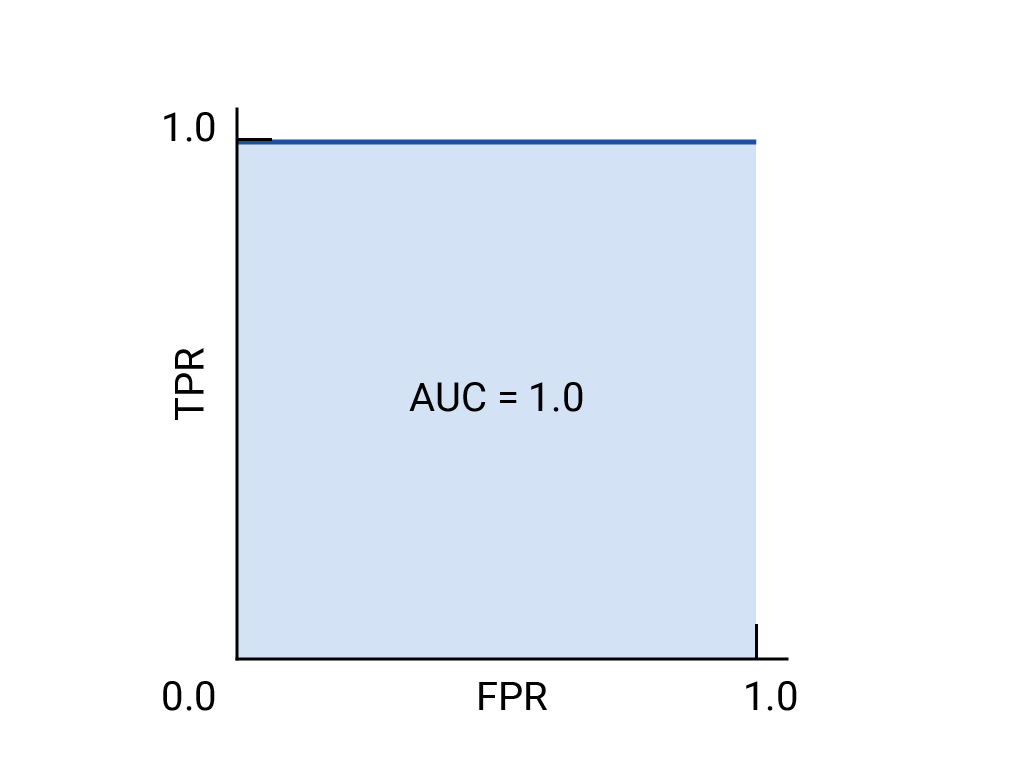
\includegraphics[width = 0.25\textwidth]{figures/schemas/auc_1-0}}
                \caption{Score AUC pour une classification naïve et une classification parfaite}
            \end{figure}

        \subsection{Score obtenu pour chaque métrique}
            \begin{table}[H]
                \centering
                \begin{tabular}{p{0.27\textwidth}|u|ddd|t|q} \toprule
                    \textbf{Modèle / Expérience} &
                \textbf{$E_{T_1, \overline C, l_{200}}$} & \textbf{$E_{T_2, \overline C, l_2}$} &
                \textbf{$E_{T_2,\overline C, l_{30}}$} & \textbf{$E_{T_2,\overline C, l_{100}}$} & \textbf{
                    $E_{T_3, C}$} & \textbf{$E_{T_4, C}$}
                    \\
                    \midrule
                    Régression logistique & 0,50 & X & 0,56 & 0,50 &  &  \\
                    Arbre de décision & 0,83 & X & 0,93 & 0,85 &  &   \\
                    Recherche des $K$ plus proches voisins & 0,63 & X & 0,79 & 0,64 &  &  \\
                    Bayésien naïf \textit{(modèle gaussien)} & 0,51 & 0,67 & 0,57 & 0,51 &  &   \\
                    Machine à vecteurs de support & 0,50 & X & 0,74 & 0,53 &  &   \\
                    Forêt aléatoire & 0,83 & X & 0,95 & 0,85 &  &  \\
                    Amplification de gradient & 0,60 & X & 0,86 & 0,73 &  &  \\
                    Empilement & 0,83 & X & 0,95 & 0,85 &  &  \\
                    \bottomrule
                \end{tabular}
                \caption{Moyenne harmonique du couple Précision-Rappel de différents classifieurs selon plusieurs configurations d'entraînement}
                \label{tab3:}
            \end{table}

            \begin{table}[H]
                \centering
                \begin{tabular}{p{0.32\textwidth}|u|ddd|tt|q} \toprule
                    \textbf{Modèle / Expérience} &
                \textbf{$E_{T_1, \overline C, l_{200}}$} & \textbf{$E_{T_2, \overline C, l_2}$} &
                \textbf{$E_{T_2,\overline C, l_{30}}$} & \textbf{$E_{T_2,\overline C, l_{200}}$} & \textbf{
                    $E_{T_3, C}$}  & \textbf{$E_{T_4, C}$} & \textbf{
                    $E_{T_4,\overline C}$} \\
                    \midrule
                    Régression logistique & 0,500 & X & 0,58 & 0,50 &  &  & \\
                    Arbre de décision & 0,499 & X & 0,78 & 0,85 &  &  & \\
                    Recherche des $K$ plus proches voisins & 0,501 & X & 0,80 & 0,64 &  &  & \\
                    Bayésien naïf \textit{(modèle gaussien)} & 0,501 & X & 0,60 & 0,51 &  &  & \\
                    Machine à vecteurs de support & 0,501 & X & 0,82 & 0,53 &  &  &  \\
                    Forêt aléatoire & 0,503 & X & 0,93 & 0,85 &  &  & \\
                    Amplification de gradient & 0,502 & X & 0,92 & 0,73 &  &  & \\
                    Empilement & 0,498 & X & 0,88 & 0,85 &  &  & \\
                    \bottomrule
                \end{tabular}
                \caption{Aire sous la courbe ROC des différents classifieurs}
                \label{tab2:}
            \end{table}

            \begin{landscape}
            \begin{table}[!ht]
                \begin{center}
                    \begin{tabular}{p{0.32\textwidth}|U|DDD|T|Q} \toprule
                    \textbf{Modèle / Expérience} & \textbf{$E_{T_1, \overline C, l_{200}}$} & \textbf{
                        $E_{T_2,\overline C, l_{2}}$} & \textbf{$E_{T_2,\overline C, l_{30}}$} & \textbf{$E_{T_2,\overline C, l_{100}}$}  & \textbf{$E_{T_3,\overline C}$} & \textbf{$E_{T_4, C}$} \\
                    \midrule
                    Régression logistique &
                    $\begin{bmatrix}0,31 & 0,19 \\ 0,32 & 0,20\end{bmatrix}$ &
                    X& $\begin{bmatrix}0,30 & 0,20 \\ 0,24 & 0,26\end{bmatrix}$  & $\begin{bmatrix}
                             0,31 & 0,19 \\
                             0,32 & 0,19\end{bmatrix}$ &
                    &   \\[3mm]
                    Arbre de décision & $\begin{bmatrix}
                                             0,26 & 0,24 \\
                                             0,26 & 0,24\end{bmatrix}$ & X&
                    $\begin{bmatrix}0,3 & 0,2 \\ 0,24 & 0,26\end{bmatrix}$ & $\begin{bmatrix}
                                                                 0,25 & 0,24 \\
                                                                 0,26 & 0,25\end{bmatrix}$ &  &   \\[3mm]
                    Recherche des $K$ plus proches voisins & $\begin{bmatrix}
                                                                 0,25 & 0,25 \\
                                                                 0,25 & 0,25\end{bmatrix}$ &
                    X& $\begin{bmatrix}0,35 & 0,15 \\ 0,13 & 0,37\end{bmatrix}$ & $\begin{bmatrix}
                                                                 0,25 & 0,24 \\
                                                                 0,25 & 0,26\end{bmatrix}$ &  &   \\
                    Bayésien naïf \textit{(modèle gaussien)} & $\begin{bmatrix}
                                                                 0,32 & 0,18 \\
                                                                 0,32 & 0,18\end{bmatrix}$ &
                    X& $\begin{bmatrix}0,31 & 0,19 \\ 0,25 & 0,26\end{bmatrix}$ & $\begin{bmatrix}
                                                                 0,32 & 0,17 \\
                                                                 0,33 & 0,18\end{bmatrix}$ &  &   \\[3mm]
                    Machine à vecteurs de support & $\begin{bmatrix}
                                                                 0,27 & 0,23 \\
                                                                 0,27 & 0,23\end{bmatrix}$ &
                    X& $\begin{bmatrix}0,37 & 0,13 \\ 0,13 & 0,37\end{bmatrix}$ & $\begin{bmatrix}
                                                                 0,30 & 0,19 \\
                                                                 0,31 & 0,2\end{bmatrix}$ &  &    \\[3mm]
                    Forêt aléatoire & $\begin{bmatrix}
                                                                 0,26 & 0,24 \\
                                                                 0,26 & 0,24\end{bmatrix}$ &
                    X& $\begin{bmatrix}0,42 & 0,08 \\ 0,08 & 0,42\end{bmatrix}$ & $\begin{bmatrix}
                                                                 0,26 & 0,23 \\
                                                                 0,27 & 0,23\end{bmatrix}$ &  &   \\[3mm]
                    Amplification de gradient & $\begin{bmatrix}
                                                                 0,25 & 0,25 \\
                                                                 0,25 & 0,25\end{bmatrix}$ &
                    X& $\begin{bmatrix}0,42 & 0,08 \\ 0,09 & 0,41\end{bmatrix}$ & $\begin{bmatrix}
                                                                 0,26 & 0,23 \\
                                                                 0,26 & 0,25\end{bmatrix}$ &  &   \\[3mm]
                    Empilement & $\begin{bmatrix}
                                     0,20 & 0,21 \\
                                     0,29 & 0,3\end{bmatrix}$ & X&
                    $\begin{bmatrix}0,41 & 0,08 \\ 0,08 & 0,42\end{bmatrix}$ & $\begin{bmatrix}
                                                                 0,20 & 0,3 \\
                                                                 0,20 & 0,31\end{bmatrix}$ &  &   \\
                    \bottomrule
                \end{tabular}
                \end{center}

                \caption{Matrices de confusion de différents classifieurs selon plusieurs configurations d'entraînement}
                \label{tab:}
            \end{table}
            \end{landscape}

    \section{Synthèse de l'utilisation des classifieurs}

    \textbf{La phase de classification de l'attaque est globalement un succès.} Les expériences
    montrent que pour une quantité suffisante de données d'entraînement, plusieurs classifieurs
    obtiennent des résultats satisfaisants, illustrés par leur métriques d'évaluation.

    \textbf{L'utilisation d'un grand nombre de modèles est intéressante car peu
    contraignante d'un point de vue de sa programmation
    \footnote{Avec \texttt{scikit-learn}, on peut utiliser une boucle itérative sur le nombre de modèles que l'on souhaite. Voir le chapitre 3 de \cite{MLFondamentaux} pour l'algorithme remanié par l'équipe.}
    et éloquente en résulats}. En effet, les performances des modèles varient d'une expérience à
    l'autre. On dégage quand-même des tendances avec une domination nette des arbres de décision,
    des forêts aléatoires, de l'amplification de gradient et plus ponctuellement de l'empilement
    de classifieurs
    \footnote{Ce résultat est par ailleurs en accord avec l'état de l'art du Machine Learning.},
    infirmant les suppositions initiales selon lesquelles un bayésien naïf ou une régression
    logistique pouvait suffir, ces modèles plus simples étant largement éprouvés lorsque l'on
    augmente $l\left(\mathbb{S}_{etr}\right)$. Pour l'ensemble des modèles, Le temps de calcul ne
    dépasse pas quelques heures si on fixe $l\left(\mathbb{S}_{etr}\right)=100000$,
    longueur pour laquelle on constate de toute façon une stagnation, voire une baisse des performances.

    À cet égard, il aurait été intéressant de dresser des courbes d'apprentissage\footnote{
    \cite{MLFondamentaux}, Chapitre 3, section 7.4} afin de déterminer la taille limite
    $l\left(\mathbb{S}_{etr}\right)$ pour laquelle les performances n'augmentent plus.

    \begin{tcolorbox}[colback=linkborder_Color!5!white,colframe=linkborder_Color!75!black]
        \textbf{Cette phase présente néanmoins un écueil important :} la précision des modèles,
        définie comme la capacité à ne pas prédire comme positif un négatif, est pour certaines
        expérimentations relativement faible. On obtient donc des classifieurs identifiant
        facilement tous les membres, mais peu fiables sur la prédiction des non-membres, avec un
        taux important de faux positifs. D'après la définition du scoring \textit{(
            \ref{Eq:scoring})} de la compétition, ce problème est donc un frein non négligeable
        à l'augmentation de $\mathtt S_{T_i}$
    \end{tcolorbox}
